\documentclass{article}
\usepackage{graphicx} % Required for inserting images
\usepackage{listings}
\usepackage{xcolor}
\lstset{
  language=Python,
  backgroundcolor=\color{gray!10}, % choose the background color; you must add \usepackage{color} or \usepackage{xcolor}
  basicstyle=\tiny\ttfamily, % the size of the fonts that are used for the code
  breaklines=false,                 % sets automatic line breaking
  breakatwhitespace=true,          % sets if automatic breaks should only happen at whitespace
  frame=single,                    % adds a frame around the code
  rulecolor=\color{black},         % if not set, the frame-color may be changed on line-breaks within not-black text (e.g. comments (green here))
  keywordstyle=\color{blue},       % keyword style
  commentstyle=\color{gray},       % comment style
  stringstyle=\color{orange},      % string literal style
  numbers=left,                    % where to put the line-numbers; possible values are (none, left, right)
  numberstyle=\tiny\color{gray},   % the style that is used for the line-numbers
  stepnumber=1,                    % the step between two line-numbers. If it's 1, each line will be numbered
  numbersep=10pt,                  % how far the line-numbers are from the code
  showspaces=false,                % show spaces everywhere adding particular underscores; it overrides 'showstringspaces'
  showstringspaces=false,          % underline spaces within strings only
  showtabs=false,                  % show tabs within strings adding particular underscores
  tabsize=2                        % sets default tabsize to 2 spaces
}

\title{Jacobi and Gauss-Seidel}
\author{QuirkyCroissant, 2024}
\date{May 2024}

\begin{document}

\maketitle

\section*{Convergence behavior of Jacobi and Gauss-Seidel}

\begin{figure}[h!]
    \centering
    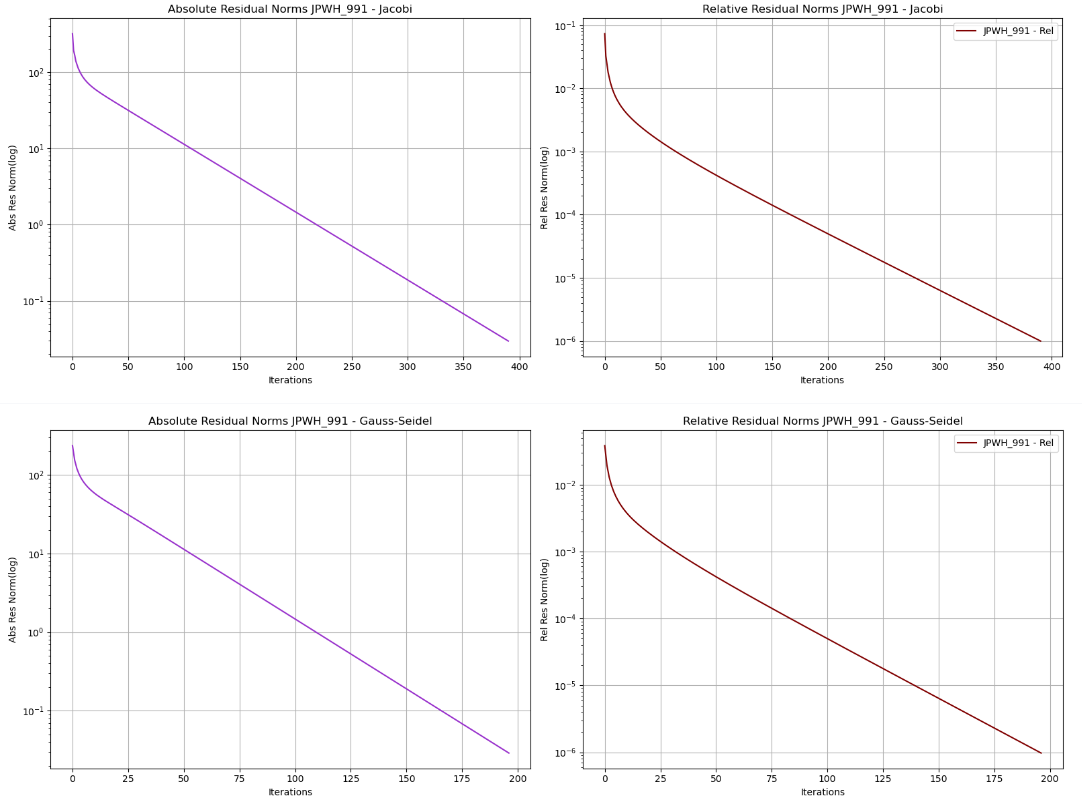
\includegraphics[width=1\linewidth]{jpwh_991_res_plot.PNG}
    \caption{JPWH\_991 Residual Plots}
\end{figure}
    For matrix "\textit{\textbf{JPWH\_991}}" the graphs for the absolute and relative residual look really similar in their behaviour for both the Jacobi as well as the Gauss-Seidel method. As the absolute residual gets rather low(10\textsuperscript{-1}) and the relative residual reaching a magnitude of 10\textsuperscript{-6}, which we defined as our tolerance of our both methods - suggests that we \textbf{reach convergance with this matrix} with both algorithms.
    
    One difference that we can observe is that with \textbf{Jacobi method} we reach the specified relative residual in 400 iterations whereas Gauss-Seidel only takes half as many iterations(200). So for "JPWH\_991" Gauss-Seidel seems to perform better. 
\begin{figure}[h!]
    \centering
    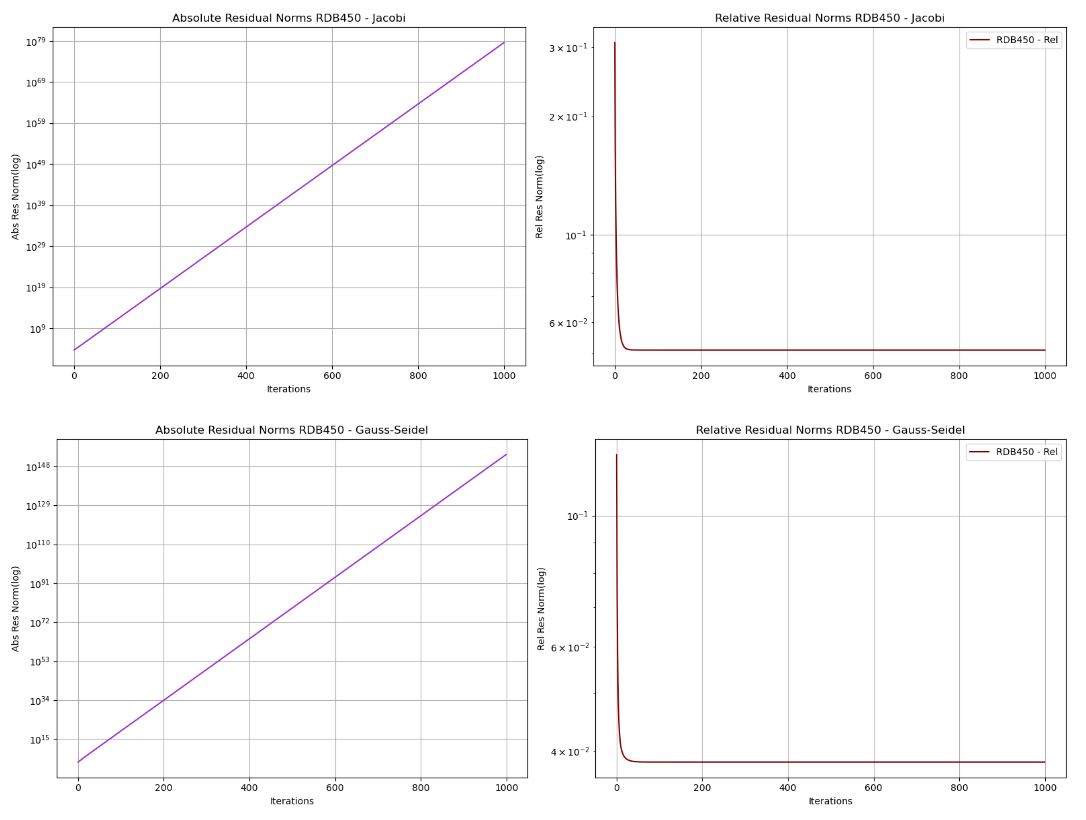
\includegraphics[width=1\linewidth]{rdb450_res_plot.PNG}
    \caption{RDB450 Residual Plots}
\end{figure}

    Again for matrix "\textbf{\textit{RDB450}}" the graphs for the absolute and relative residual look really similar in their behaviour for both the Jacobi as well as the Gauss-Seidel method. But a key difference to the results with the last matrix is that the absolute residual starts rather high and further increases by the number of iterations until we reach our iteration limit of 1000, which is a\textbf{ strong characteristic of divergence}(10\textsuperscript{79} and 10\textsuperscript{148}). The graph of the relative residual shows that for one we never reach our goal of 10\textsuperscript{-6} relative residual, but also it seems that it gets a tiny bit better at first after a few iterations before our relative residual begins to stagnate at 4 or 6 * 10\textsuperscript{-2} respectively and never gets better onward. 
    Both methods do not converge, and although the relative residual of the \textbf{Gauss-Seidel} shows a maginally lower residual at iteration 1000(4 * 10\textsuperscript{-2}), I am hesident to call it "better" because both methods fail to converge and get us a satisfying result.
\begin{figure}[h!]
    \centering
    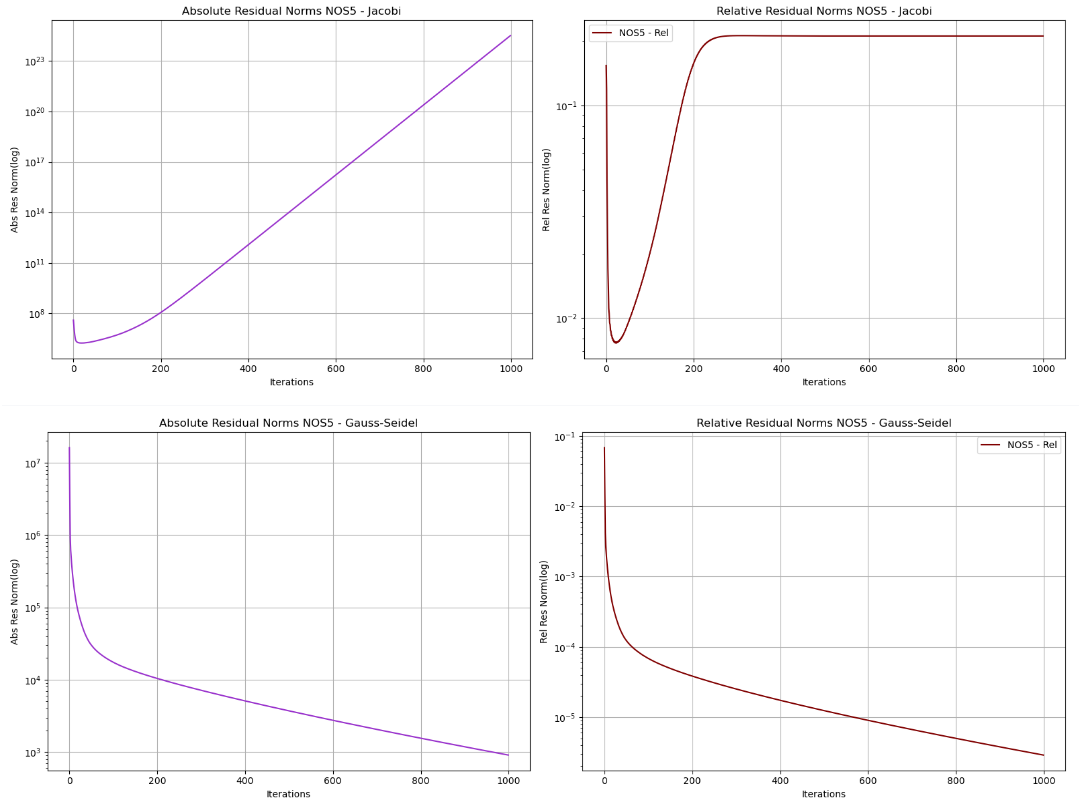
\includegraphics[width=1\linewidth]{nos5_res_plot.PNG}
    \caption{NOS5 Residual Plots}
\end{figure}
    \pagebreak
    
    The plots for matrix "\textbf{\textit{NOS5}}" get interesting, because this time we can observe completely different behaviours for our iterative methods. When applying the Jacobi Methode on the given matrix, we can see that the absolute residual starts high but decreases at the beginning, before changing its trend drastically and increases exponentially after certain iterations(absolute residual intervall [10\textsuperscript{6}, ~10\textsuperscript{23}]). If we look at the relative residual we can see a similar behaviour, where our accuracy improves at the beginning before skyrocketing again after some iterations before it starts to stagnate at about slightly above  10\textsuperscript{-1}. Both metrics suggest \textbf{divergence}.
    When we look at the results of Gauss-Seidel, we can see a completely different picture. Looking at the absolute residual, we first start at a high absolute residual(10\textsuperscript{7}) before steadily decreasing significantly. Same trend can be observed with the relative residual which starts at 10\textsuperscript{-1} and improves steadily till 10\textsuperscript{-5}. Both \textbf{trends suggest convergance}, but we can see that we will not reach our desired tolerance of 10\textsuperscript{-6} in under 1000 iterations, therefore also the \textbf{Gauss-Seidel} approach fails to achieve that - but it suggest convergance after certain alternative conditions(increase iterations, preprocessing the input matrix etc), therefore a significant improvement to the Jacobi Methode in this case.
    
    Throughout the 2 later matrixes the relative residuals showed different trends to the absolute residual variant. I would explain it as such, that that phenomena occurs, because of the normalization of the discrepancy of our approximation to the true solution in the relative residual (among others). While the former shows the absolute error magnitude without normalization it can also be rather sensitive of certain scales. But the relative residual can also like descriped before can show initial improvements before growing exponentially again, in case of convergence(while the absolute residual steadily increases in a linear manner).
    
\section*{Reason for convergence respectively divergence}

A rather important metric to signify if a specific iteration matrix G leads to convergence or not seems to be the spectral radius. We get this property by retrieving the largest absolut eigenvalue form our iteration matrix G. We interpret the results as following if:\newline
$$\rho(G) < 1 \; convergance$$
$$\rho(G) \geq 1 \; divergence$$
if we now compute the iteration matrix G for every Jacobi or Gauss-Seidel application and retrieve there respective eigenvalues in correlation to the test matrices we get the following result, which perfectly mimics the behavior of each descript above. 
 \begin{figure}[h!]
     \centering
     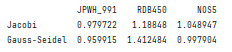
\includegraphics[width=0.5\linewidth]{spec_radii_stats.PNG}
     \caption{spectral radii for the test matrices}
 \end{figure}
\begin{figure}
    \centering
    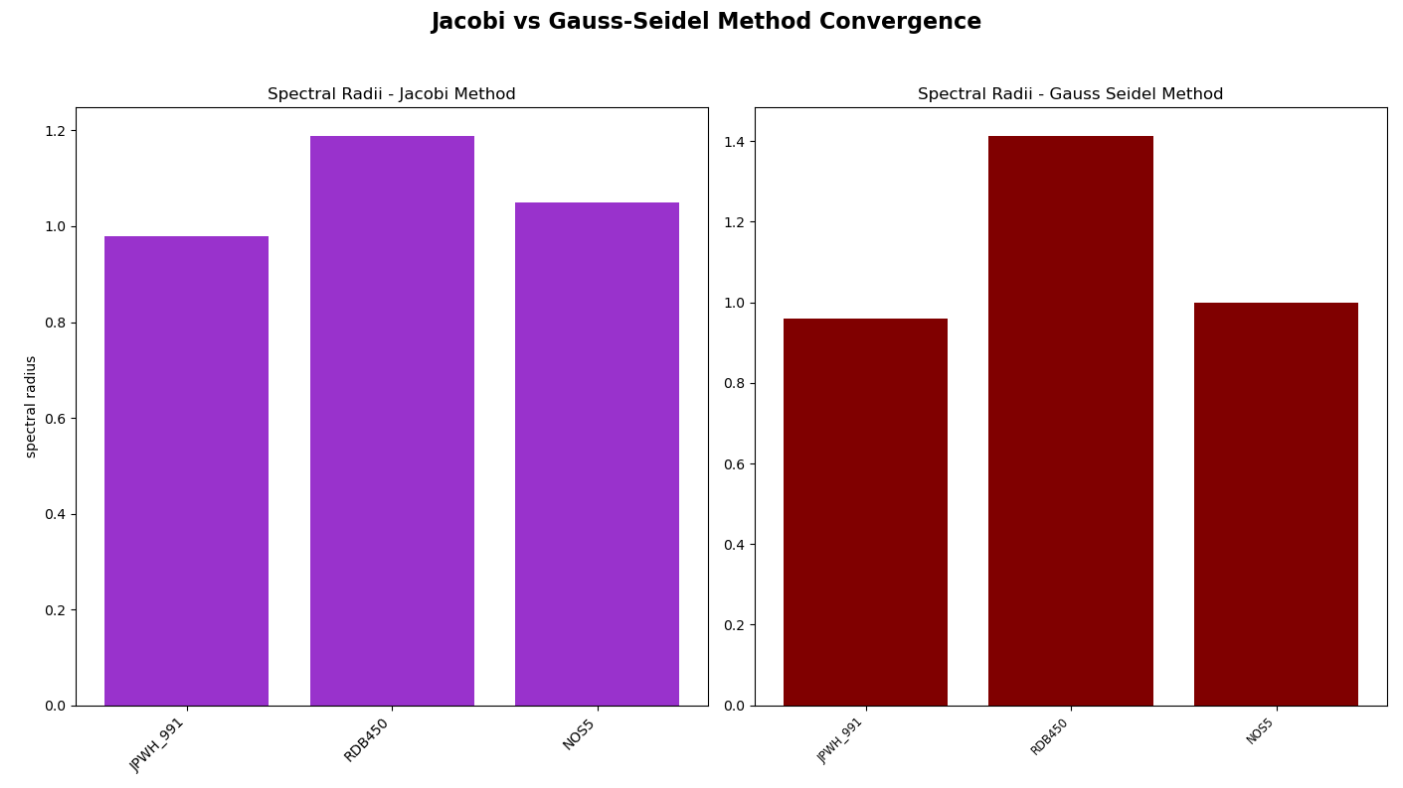
\includegraphics[width=1\linewidth]{spec_radii_bar_plot.PNG}
    \caption{spectral radii bar plot}
\end{figure}

\end{document}

